\chapter{MÔ TẢ TỔNG QUAN HỆ THỐNG}

\section{Bối cảnh hệ thống}
Trong các trung tâm dữ liệu và phòng máy chủ, việc giám sát cơ sở hạ tầng thường được thực hiện thông qua các bảng điều khiển (dashboard) trên nền tảng web và các hệ thống quản lý tập trung. Các hệ thống này cung cấp thông tin về mức sử dụng tài nguyên (CPU, RAM, Disk, Traffic), trạng thái máy chủ và cảnh báo tức thời. Tuy nhiên, dữ liệu giám sát chủ yếu tồn tại dưới dạng thông tin số hiển thị trên màn hình máy tính và bị tách biệt hoàn toàn với vị trí vật lý của thiết bị trong không gian thực.

Khi xảy ra sự cố, kỹ thuật viên phải đối chiếu thủ công thông tin cảnh báo trên dashboard với sơ đồ mặt bằng tủ rack để định vị máy chủ gặp sự cố. Việc tìm kiếm thiết bị giữa hàng trăm máy chủ có ngoại hình giống hệt nhau, kiểm tra workload, xác minh cáp nối vật lý và tra cứu lịch sử sửa chữa làm tăng đáng kể chỉ số MTTR (Mean Time to Resolution). Thêm vào đó, kỹ thuật viên làm việc tại hiện trường không thể truy cập trực tiếp các thông số telemetry và nhật ký dịch vụ thời gian thực ngay tại vị trí đặt máy chủ.

Hệ thống \textbf{AR-IMMS} được đề xuất để giải quyết triệt để rào cản này bằng cách kết nối cơ sở hạ tầng vật lý với dữ liệu vận hành kỹ thuật số thông qua mô hình Digital Twin, telemetry thời gian thực và công nghệ Thực tế Tăng cường (AR). Mô hình Digital Twin biểu diễn cấu trúc phân cấp hạ tầng, trong khi ứng dụng di động AR giúp kỹ thuật viên nhận diện chính xác máy chủ vật lý bằng QR/ArUco Marker và hiển thị trực quan các lớp dữ liệu vận hành (overlay) ngay trên camera thiết bị.

Do hạn chế về điều kiện thử nghiệm thực tế tại Data Center thương mại, hệ thống AR-IMMS được triển khai và đánh giá trên mô hình \textbf{Mini Data Center Testbed}. Cụm các máy tính vật lý đóng vai trò là Server/Node, các nhóm máy tính đóng vai trò là Rack, và các ứng dụng/dịch vụ container hóa đóng vai trò là Workload.

\section{Mục tiêu của hệ thống}
Mục tiêu tổng quát của AR-IMMS là xây dựng một nền tảng quản lý tập trung khép kín, nâng cao hiệu quả giám sát, rút ngắn thời gian phát hiện và xử lý sự cố, đồng thời tối ưu hóa quy trình bảo trì hạ tầng Data Center.

\subsection{Mô hình hóa cơ sở hạ tầng bằng Digital Twin}
Xây dựng mô hình Digital Twin phân cấp theo cấu trúc chuẩn:
\begin{equation*}
\text{Site} \longrightarrow \text{Room} \longrightarrow \text{Rack} \longrightarrow \text{Node/Server} \longrightarrow \text{Container/Workload}
\end{equation*}
Cho phép người dùng theo dõi vị trí không gian, mối quan hệ phụ thuộc và trạng thái sức khỏe kỹ thuật số của từng thành phần trong toàn bộ hệ thống.

\subsection{Giám sát Telemetry thời gian thực}
Thu thập tự động các chỉ số vận hành phần cứng (CPU, RAM, Nhiệt độ, Disk, Network) và thông số Docker container từ các máy chủ thông qua Monitoring Agent. Truyền dữ liệu trực tiếp về Web Command Center bằng chuẩn giao tiếp WebSocket/Socket.IO với chu kỳ 5 giây.

\subsection{Kết nối dữ liệu số với thiết bị vật lý qua AR}
Định danh các nút máy chủ vật lý bằng mã QR hoặc ArUco Marker. Kỹ thuật viên hiện trường sử dụng ứng dụng di động AR để quét marker, nhận diện thiết bị và xem lớp phủ dữ liệu (telemetry, trạng thái sức khỏe, log dịch vụ) hiển thị khớp với không gian thực tế của máy chủ.

\subsection{Phát hiện và xử lý sự cố tự động}
Hệ thống tự động so sánh dữ liệu thu thập với các ngưỡng cảnh báo cấu hình trước (ví dụ: CPU $> 90\%$, Nhiệt độ $> 75^\circ\text{C}$ hoặc Mất kết nối $> 90\text{s}$). Tự động khởi tạo Alert, lọc bỏ trùng lặp (Alert Storm Suppression) và chuyển đổi thành Incident/Ticket để phân công xử lý.

\subsection{Hỗ trợ quản lý bảo trì và kiểm toán}
Phân công phiếu bảo trì (Ticket) cho kỹ thuật viên, theo dõi tiến độ thực hiện tại hiện trường, thực hiện xác thực thao tác nguy hiểm (Step-up Verification) và ghi nhận nhật ký kiểm toán không thể sửa xóa (Immutable Audit Log) phục vụ đánh giá tuân thủ và phân tích hiệu suất năng lượng (PUE).

\section{Các bên liên quan (Stakeholders \& Actors)}
Hệ thống AR-IMMS bao gồm 4 nhóm tác nhân (Actors) tương tác chính:

\begin{figure}[H]
    \centering
    \begin{tabular}{|p{3.5cm}|p{11cm}|}
    \hline
    \textbf{Tác nhân (Actor)} & \textbf{Mô tả vai trò và trách nhiệm} \\ \hline
    \textbf{Quản trị viên (Administrator)} & Chịu trách nhiệm quản trị người dùng (tạo, khóa, phân quyền RBAC), cấu hình thiết lập hệ thống, theo dõi tổng quan sức khỏe dịch vụ backend, quản lý cấu hình Mini Data Center và tra cứu nhật ký kiểm toán (Audit Log). \\ \hline
    \textbf{Chuyên viên Vận hành (System Operator)} & Người vận hành trung tâm chỉ huy hằng ngày. Quản lý danh mục tài sản hạ tầng, gán mã QR/ArUco cho máy chủ, giám sát bảng điều khiển thời gian thực, xem sơ đồ Digital Twin, thiết lập ngưỡng cảnh báo, xác nhận Alert, khởi tạo và phân công Ticket bảo trì, duyệt đóng Ticket và xuất báo cáo vận hành/PUE. \\ \hline
    \textbf{Kỹ thuật viên hiện trường (Field Technician)} & Người tiếp nhận Ticket bảo trì, di chuyển đến phòng máy, sử dụng ứng dụng Mobile AR để quét nhận diện thiết bị, xem telemetry và cảnh báo trực quan tại chỗ, thực hiện thao tác sửa chữa/bảo trì, cập nhật ghi chú sự cố và gửi yêu cầu đóng Ticket. \\ \hline
    \textbf{Monitoring Agent (System Actor)} & Thành phần phần mềm tự động chạy ngầm trên từng máy chủ. Thu thập thông số phần cứng, OS và Docker container, đóng gói dữ liệu và gửi liên tục về Backend API qua kết nối an toàn mTLS / WebSocket. \\ \hline
    \end{tabular}
    \caption{Bảng tóm tắt các tác nhân trong hệ thống AR-IMMS}
\end{figure}

\section{Phạm vi chức năng và Kiến trúc tổng quan}
Phạm vi chức năng phần mềm AR-IMMS được phân chia thành 10 nhóm mô-đun chính:

\begin{table}[H]
\centering
\begin{tabularx}{\textwidth}{|l|X|}
\hline
\textbf{Nhóm mô-đun} & \textbf{Nội dung chi tiết} \\ \hline
Xác thực \& Phân quyền & Đăng nhập, đăng xuất, đổi mật khẩu, cấp phát JWT Token, kiểm soát truy cập dựa trên vai trò (RBAC). \\ \hline
Quản lý Hạ tầng & Quản lý cấu trúc cây không gian: Site, Room, Rack, Server vàWorkload. Liên kết mã định danh QR/ArUco. \\ \hline
Giám sát \& Telemetry & Thu thập chỉ số phần cứng/OS/Docker, hiển thị đồ thị thời gian thực, phát hiện ngắt kết nối (Agent timeout). \\ \hline
Digital Twin Engine & Dựng mô hình số của Data Center, trực quan hóa trạng thái sức khỏe, đồng bộ liên tục dữ liệu telemetry. \\ \hline
Quản lý Cảnh báo & Tự động phát hiện vượt ngưỡng, lọc trùng lặp Alert, quản lý vòng đời (Open, Acknowledged, Resolved, Closed). \\ \hline
Quản lý Sự cố & Tạo Incident từ Alert, gắn thông tin thiết bị, phân công người chịu trách nhiệm và theo dõi xử lý. \\ \hline
Quản lý Bảo trì & Tạo phiếu công việc (Ticket), giao cho Technician, cập nhật tiến độ và quy trình nghiệm thu đóng Ticket. \\ \hline
Quản lý Tài sản \& Bảo hành & Quản lý thông số phần cứng chi tiết, ngày mua, hạn bảo hành, lịch sử thay thế linh kiện và kiểm toán. \\ \hline
Ứng dụng Mobile AR & Quét mã định danh, nhận diện thiết bị, hiển thị lớp phủ thông số thời gian thực, xác thực 2 bước cho hành động can thiệp. \\ \hline
Báo cáo \& Kiểm toán & Thống kê telemetry lịch sử, báo cáo sự cố/Ticket, phân tích chỉ số hiệu năng PUE và xuất nhật ký Audit Log. \\ \hline
\end{tabularx}
\caption{Phân vùng phạm vi chức năng của hệ thống AR-IMMS}
\end{table}

\section{Giả định và Ràng buộc}

\subsection{Giả định hệ thống}
\begin{itemize}
    \item Cụm máy tính thuộc Mini Data Center Testbed có kết nối mạng LAN/Intranet ổn định đến cụm server Backend.
    \item Mỗi nút máy chủ vật lý được cài đặt sẵn Monitoring Agent phù hợp với hệ điều hành đang chạy.
    \item Tất cả các máy chủ vật lý phục vụ tính năng AR đã được dán mã QR/ArUco Marker chính xác ở vị trí dễ quét phía trước vỏ máy.
    \item Kỹ thuật viên hiện trường được trang bị thiết bị di động chạy hệ điều hành Android (phiên bản $\ge 8.0$) có camera hỗ trợ tự động lấy nét và kết nối Wi-Fi nội bộ.
    \item Các ngưỡng cảnh báo mặc định đã được Operator định cấu hình trước khi kích hoạt quy trình phát hiện sự cố.
\end{itemize}

\subsection{Ràng buộc hệ thống}
\begin{enumerate}
    \item \textbf{Môi trường triển khai:} Hệ thống được thiết kế cho mô hình thử nghiệm Mini Data Center Testbed, chưa hỗ trợ trực tiếp các giao thức quản lý công nghiệp chuyên dụng như IPMI hoặc SNMP trong phiên bản hiện tại.
    \item \textbf{Thời gian thực và Telemetry:} Chu kỳ gửi dữ liệu mặc định của Agent là 5 giây. Nếu trong thời gian 90 giây liên tục Backend không nhận được dữ liệu từ một Agent, máy chủ đó bắt buộc phải bị đánh dấu là \textit{Unavailable}.
    \item \textbf{Bảo mật và Kiểm toán:} Kết nối truyền dữ liệu giữa Agent và Backend bắt buộc mã hóa qua mTLS. Mọi thao tác cấu hình hệ thống, giao việc và can thiệp từ xa trên app AR bắt buộc phải ghi lại trong nhật ký kiểm toán (Audit Log) cố định.
    \item \textbf{Công nghệ áp dụng:}
    \begin{itemize}
        \item Backend API: NestJS / Python FastAPI (RESTful \& Socket.IO Gateway).
        \item Web Command Center: Next.js / React (Định dạng Desktop-first, ưu tiên giao diện tiếng Anh).
        \item Mobile App: React Native tích hợp thư viện Computer Vision / AR (Android OS).
        \item Định danh vật lý: Chuẩn mã QR Code và ArUco Marker nhị phân.
    \end{itemize}
    \item \textbf{Khả năng mở rộng (Scalability constraint):} Khi một nút máy chủ mới được đăng ký và cài đặt Agent, thiết bị phải tự động stream telemetry và xuất hiện trên giao diện Digital Twin trong vòng dưới 5 phút mà không cần khởi động lại hoặc sửa đổi mã nguồn Backend.
\end{enumerate}

\section{Mô hình Thực thể - Mối quan hệ (ERD)}
Mô hình dữ liệu của hệ thống AR-IMMS được thiết kế nhằm quản lý toàn diện cấu trúc cơ sở hạ tầng phân cấp Digital Twin, chuỗi dữ liệu telemetry thời gian thực, quy trình cảnh báo - ticket khép kín và nhật ký kiểm toán bất biến.

\begin{figure}[H]
    \centering
    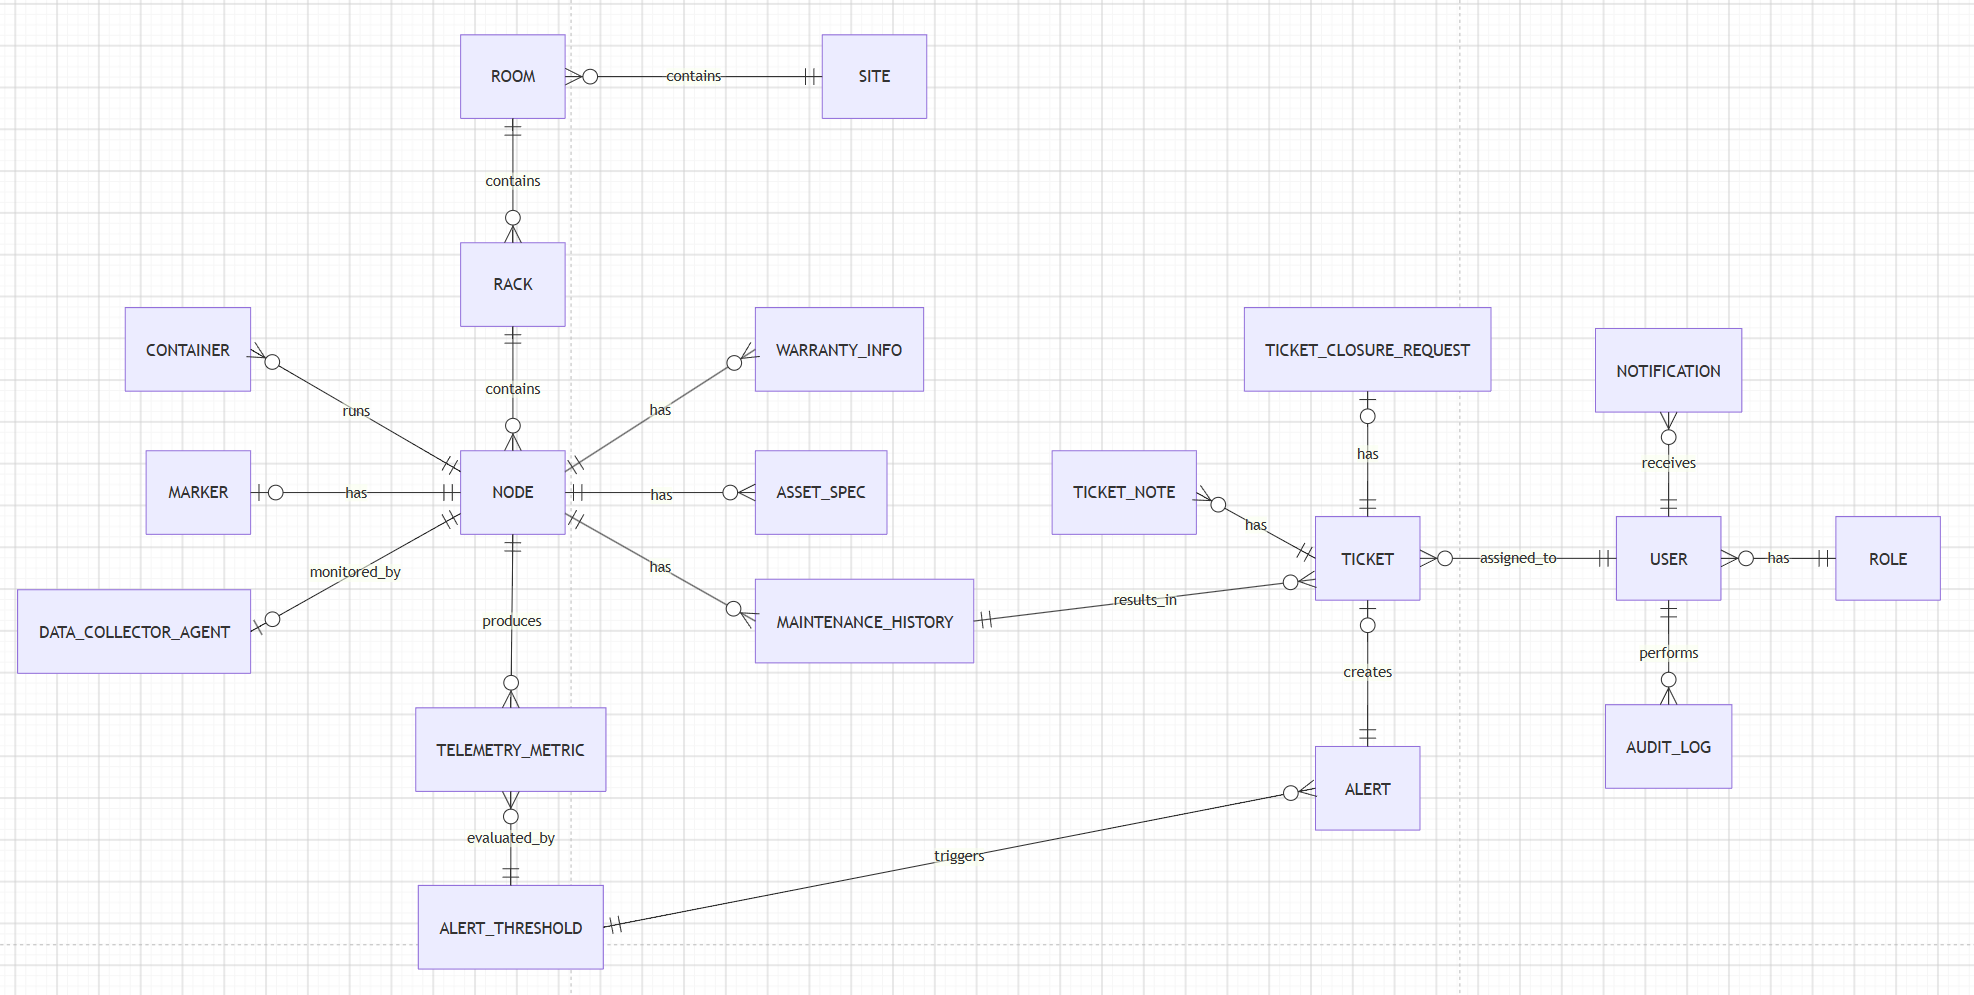
\includegraphics[width=0.98\textwidth]{ERD.png}
    \caption{Sơ đồ Thực thể - Mối quan hệ (ERD) hệ thống AR-IMMS}
    \label{fig:erd_diagram}
\end{figure}

\subsection{Phân tích các Thực thể chính (Entities)}
Hệ thống bao gồm 15 thực thể chính được nhóm thành 5 phân hệ dữ liệu cốt lõi:
\begin{enumerate}
    \item \textbf{Phân hệ Người dùng \& Kiểm toán:}
    \begin{itemize}
        \item \texttt{User}: Lưu trữ thông tin tài khoản, mật khẩu mã hóa (hash), vai trò RBAC (\textit{ADMINISTRATOR}, \textit{SYSTEM\_OPERATOR}, \textit{FIELD\_TECHNICIAN}) và họ tên.
        \item \texttt{AuditLog}: Ghi lại nhật ký tác động hệ thống bất biến (User ID, Thao tác, Loại tài nguyên, ID tài nguyên, Chi tiết JSON, IP Address, Timestamp).
    \end{itemize}
    \item \textbf{Phân hệ Cấu trúc Hạ tầng Digital Twin:}
    \begin{itemize}
        \item \texttt{Site}: Lưu thông tin các vị trí trung tâm dữ liệu (Mã, Tên, Địa điểm, Mô tả).
        \item \texttt{Room}: Lưu thông tin phòng máy thuộc Site (Mã, Tên, Tầng).
        \item \texttt{Rack}: Lưu thông tin tủ rack thuộc Room (Mã, Tên, Sức chứa Unit capacity, Năng lượng tối đa).
        \item \texttt{Node}: Lưu thông tin các máy chủ server thuộc Rack (Tên, Hostname, IP, MAC Address, Trạng thái ONLINE/OFFLINE/WARNING/CRITICAL, Vị trí U, Công suất tiêu thụ).
        \item \texttt{Container}: Lưu thông tin các workload/Docker container chạy trên Node (Container ID, Tên, Image, CPU\%, RAM usage, Trạng thái RUNNING/STOPPED, Số lần restart).
    \end{itemize}
    \item \textbf{Phân hệ Định danh AR \& Telemetry Agent:}
    \begin{itemize}
        \item \texttt{Marker}: Lưu mã định danh QR/ArUco Marker gán cho Node, loại marker và tọa độ không gian 3D dạng JSON.
        \item \texttt{DataCollectorAgent}: Lưu thông tin phần mềm Agent thu thập telemetry cài trên Node (Phiên bản, Trạng thái ACTIVE/INACTIVE, API Key Hash, Last Heartbeat).
        \item \texttt{TelemetryMetric}: CSDL chuỗi thời gian lưu dữ liệu đo đạc (CPU\%, RAM\%, Disk\%, Nhiệt độ, Network Rx/Tx, Timestamp).
    \end{itemize}
    \item \textbf{Phân hệ Cảnh báo, Sự cố \& Bảo trì:}
    \begin{itemize}
        \item \texttt{Alert}: Lưu cảnh báo bất thường từ Node (Loại chỉ số, Giá trị ngưỡng, Giá trị thực tế, Mức độ WARNING/CRITICAL, Trạng thái OPEN/ACKNOWLEDGED/RESOLVED/CLOSED, Số lần lặp lại occurrence count).
        \item \texttt{Ticket}: Lưu phiếu công việc bảo trì (Alert ID liên kết, Node ID, Tiêu đề, Mô tả, Mức ưu tiên LOW/MEDIUM/HIGH/CRITICAL, Trạng thái OPEN/ASSIGNED/IN\_PROGRESS/RESOLVED/CLOSED, ID người tạo, ID người được gán).
        \item \texttt{TicketNote}: Ghi chú diễn biến xử lý ticket từ kỹ thuật viên (Ticket ID, Author User ID, Nội dung ghi chú, Thời gian).
        \item \texttt{TicketClosureRequest}: Yêu cầu nghiệm thu đóng ticket từ Technician (Summary, Chi tiết xử lý, Trạng thái PENDING/APPROVED/REJECTED, ID người duyệt).
        \item \texttt{MaintenanceHistory}: Lịch sử bảo trì phục vụ kiểm toán thiết bị (Node ID, Ticket ID, Loại bảo trì, Mô tả, Người thực hiện, Thời gian).
    \end{itemize}
    \item \textbf{Phân hệ Thông số Kỹ thuật \& Bảo hành:}
    \begin{itemize}
        \item \texttt{AssetSpec}: Lưu cấu hình phần cứng chi tiết của Node (CPU Model, Cores, RAM GB, Storage GB, OS Name, OS Version).
        \item \texttt{WarrantyInfo}: Lưu thông tin bảo hành máy chủ (Vendor, Model Number, Serial Number, Ngày mua, Ngày bắt đầu/kết thúc bảo hành, Đơn vị hỗ trợ).
    \end{itemize}
\end{enumerate}

\subsection{Phân tích Mối quan hệ giữa các Thực thể (Entity Relationships)}
Bảng dưới đây tổng hợp bản chất mối quan hệ, khóa ngoại (Foreign Key) và quy tắc ràng buộc giữa các thực thể:

\begin{longtable}{|p{3cm}|p{3cm}|p{2.5cm}|p{5cm}|}
\hline
\textbf{Thực thể Cha} & \textbf{Thực thể Con} & \textbf{Tỷ lệ (Card.)} & \textbf{Khóa ngoại (FK) \& Diễn giải} \\ \hline
\endhead
\texttt{Site} & \texttt{Room} & $1 : N$ & \texttt{Room.site\_id} $\rightarrow$ Một Site chứa nhiều Room. \\ \hline
\texttt{Room} & \texttt{Rack} & $1 : N$ & \texttt{Rack.room\_id} $\rightarrow$ Một Room chứa nhiều tủ Rack. \\ \hline
\texttt{Rack} & \texttt{Node} & $1 : N$ & \texttt{Node.rack\_id} $\rightarrow$ Một Rack chứa nhiều máy chủ Node. \\ \hline
\texttt{Node} & \texttt{Container} & $1 : N$ & \texttt{Container.node\_id} $\rightarrow$ Một Node chạy nhiều Container workload. \\ \hline
\texttt{Node} & \texttt{Marker} & $1 : N$ & \texttt{Marker.node\_id} $\rightarrow$ Một Node có các mã AR Marker định danh. \\ \hline
\texttt{Node} & \texttt{DataCollectorAgent} & $1 : N$ & \texttt{DataCollectorAgent.node\_id} $\rightarrow$ Một Node cài Agent thu thập. \\ \hline
\texttt{Node} & \texttt{TelemetryMetric} & $1 : N$ & \texttt{TelemetryMetric.node\_id} $\rightarrow$ Lưu chuỗi bản tin telemetry. \\ \hline
\texttt{Node} & \texttt{Alert} & $1 : N$ & \texttt{Alert.node\_id} $\rightarrow$ Phát sinh các cảnh báo cho Node. \\ \hline
\texttt{Alert} & \texttt{Ticket} & $0..1 : N$ & \texttt{Ticket.alert\_id} $\rightarrow$ Chuyển đổi cảnh báo thành Ticket. \\ \hline
\texttt{Node} & \texttt{Ticket} & $1 : N$ & \texttt{Ticket.node\_id} $\rightarrow$ Ticket gắn liền với thiết bị mục tiêu. \\ \hline
\texttt{User} & \texttt{Ticket} & $1 : N$ & \texttt{Ticket.created\_by\_user\_id}, \texttt{assigned\_to\_user\_id}. \\ \hline
\texttt{Ticket} & \texttt{TicketNote} & $1 : N$ & \texttt{TicketNote.ticket\_id} $\rightarrow$ Các ghi chú xử lý công việc. \\ \hline
\texttt{Ticket} & \texttt{TicketClosureRequest} & $1 : 0..1$ & \texttt{TicketClosureRequest.ticket\_id} $\rightarrow$ Yêu cầu đóng ticket. \\ \hline
\texttt{Node} & \texttt{MaintenanceHistory} & $1 : N$ & \texttt{MaintenanceHistory.node\_id} $\rightarrow$ Nhật ký lịch sử bảo trì. \\ \hline
\texttt{Node} & \texttt{AssetSpec} & $1 : 1$ & \texttt{AssetSpec.node\_id} $\rightarrow$ Thông số phần cứng chi tiết Node. \\ \hline
\texttt{Node} & \texttt{WarrantyInfo} & $1 : 1$ & \texttt{WarrantyInfo.node\_id} $\rightarrow$ Hồ sơ bảo hành thiết bị. \\ \hline
\texttt{User} & \texttt{AuditLog} & $1 : N$ & \texttt{AuditLog.user\_id} $\rightarrow$ Nhật ký kiểm toán thao tác người dùng. \\ \hline
\end{longtable}

